\chapter{Implementaci\'on del prototipo}
\label{chap:implementacion}

La implementaci\'on se entrega como un repositorio reproducible con tres piezas separadas: la aplicaci\'on Angular, un backend \emph{backend for frontend} (BFF) escrito en Node.js/Express y un paquete de configuraci\'on documental para Copilot Studio. La separaci\'on permite revisar cada frontera de seguridad y evita que los pasos que requieren un tenant de Microsoft queden ocultos en el c\'odigo.

\section{Tecnolog\'ias y estructura del proyecto}

Angular se utiliza para la experiencia de usuario por su tipado mediante TypeScript, su mecanismo de sanitizaci\'on y su arquitectura de componentes. El BFF asume funciones que no deben realizarse en el navegador: validar configuraci\'on, aplicar controles de tasa y solicitar un token temporal al servicio Direct Line. La biblioteca Bot Framework Web Chat se integra en un contenedor del cliente y recibe solamente el token temporal. El agente se administra en Copilot Studio, donde residen las instrucciones, fuentes, temas y configuraci\'on de publicaci\'on.

La estructura de entrega mantiene el material acad\'emico y el ejecutable separados:

\begin{lstlisting}[caption={Estructura l\'ogica del repositorio.},label={lst:estructura}]
apps/
  web/              # Cliente Angular
  api/              # BFF: token Direct Line y health check
copilot-agent/
  INSTRUCCIONES_AGENTE.md
  temas/            # Dise\~no de temas para importar/configurar
  conocimiento/     # Inventario y res\'umenes aprobados
  pruebas/          # Casos sint\'eticos y r\'ubrica
memoria/            # Fuente LaTeX y anexos
evidencias/         # Salidas de validaci\'on reproducibles
\end{lstlisting}

Fijar las versiones de dependencias y conservar un archivo de bloqueo permite repetir la compilaci\'on. Antes de publicar deben ejecutarse auditor\'ias de dependencias y comprobarse que los artefactos no incluyen archivos \texttt{.env}, secretos o datos de pruebas sensibles. El prototipo no usa Docker como requisito de ejecuci\'on, aunque puede contener una configuraci\'on de despliegue posterior.

\section{Configuraci\'on del agente en Copilot Studio}

La configuraci\'on se realiza en un entorno de desarrollo de Copilot Studio al que el propietario tenga permisos. La licencia y el acceso son requisitos de plataforma, no elementos que puedan simularse en el repositorio \cite{copilotLicensing}. La secuencia reproducible es la siguiente:

\begin{enumerate}[label=\arabic*.]
  \item Crear un agente en blanco en espa\~nol con el prop\'osito limitado a orientaci\'on de ciberseguridad.
  \item Activar la orquestaci\'on generativa y copiar las instrucciones versionadas del paquete entregado. Solo se mencionan conocimientos, temas y herramientas que est\'an realmente configurados, seg\'un exige la plataforma \cite{copilotInstructions}.
  \item Cargar las fuentes aprobadas o registrar las URL institucionales seleccionadas. Durante la evaluaci\'on se desactiva la b\'usqueda web abierta y la opci\'on de respuestas no fundamentadas, cuando las pol\'iticas del tenant lo permitan \cite{copilotKnowledge}.
  \item Crear los temas de derivaci\'on, rechazo, phishing, incidentes y feedback a partir de sus descripciones y flujos. Los temas de riesgo aplican pasos deterministas.
  \item Probar cada tema en el panel de pruebas, documentar la versi\'on y publicar solo cuando la matriz de regresi\'on sea satisfactoria.
  \item Configurar el canal web para acceso seguro y anotar el secreto Direct Line exclusivamente en la variable de entorno del BFF. El secreto no se copia en la configuraci\'on Angular.
\end{enumerate}

El paquete \texttt{copilot-agent} no finge ser una exportaci\'on de soluci\'on de Power Platform, cuyo formato depende del tenant y de la versi\'on de la plataforma. En cambio, proporciona los textos, inventarios y flujos que se deben revisar antes de crear o importar elementos en el portal. Esta decisi\'on evita declarar como desplegable un archivo con un esquema no verificado.

\section{Instrucciones y pol\'itica de comportamiento}

Las instrucciones del agente se organizan en seis capas: identidad y alcance; prioridades de evidencia; tratamiento de incertidumbre; seguridad y privacidad; respuesta a consultas potencialmente da\~ninas; y estilo de comunicaci\'on. El orden de prioridad es: preservar la seguridad, respetar los l\'imites, basar los hechos en las fuentes aprobadas y, por \`ultimo, maximizar la utilidad. Esta jerarqu\'ia es preferible a una instrucci\'on gen\'erica de ``responder siempre'', que fomentar\'ia alucinaciones cuando no existe cobertura.

Una respuesta dentro de alcance debe contener: una conclusi\'on breve, pasos reversibles o de bajo riesgo, advertencias relevantes y cita. Si no hay evidencia suficiente, el agente declara la limitaci\'on, explica qu\'e dato m\'inimo permitir\'ia orientar la consulta y sugiere un canal humano. Ante indicios de incidente, la salida se limita a medidas prudentes de preservaci\'on y notificaci\'on; no solicita muestras, credenciales ni informaci\'on interna. Estas reglas se verifican de forma expl\'icita en los casos de prueba adversarios.

\section{Integraci\'on segura mediante Direct Line}

Una integraci\'on directa en una SPA que incluye un secreto constituye una vulnerabilidad de dise\~no: cualquier persona que abra las herramientas de desarrollo puede reutilizarlo. Por ello, el flujo de la figura \ref{fig:secuencia-token} delega el canje de secreto a token en el BFF. La web recibe un token por conversaci\'on, no el secreto permanente. Microsoft documenta que los tokens de Direct Line son espec\'ificos de la conversaci\'on y expiran \cite{copilotDirectLine}.

\begin{figure}[H]
\centering
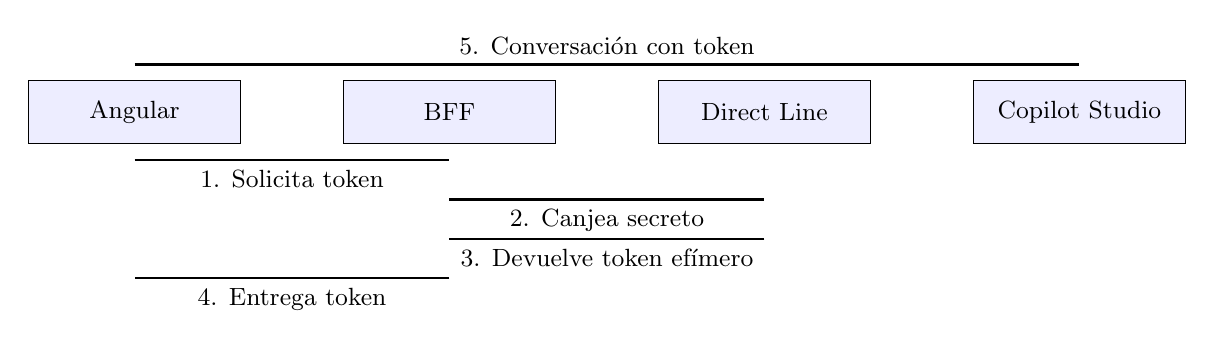
\begin{tikzpicture}[
  every node/.style={font=\small},
  actor/.style={draw, fill=blue!7, minimum width=27mm, minimum height=8mm, align=center},
  arrow/.style={thick}
]
\node[actor] (spa) at (0,0) {Angular};
\node[actor] (bff) at (4,0) {BFF};
\node[actor] (direct) at (8,0) {Direct Line};
\node[actor] (agent) at (12,0) {Copilot Studio};
\draw[arrow] (spa.south) ++(0,-.2) -- ++(4,0) node[midway, below]{1. Solicita token};
\draw[arrow] (bff.south) ++(0,-.7) -- ++(4,0) node[midway, below]{2. Canjea secreto};
\draw[arrow] (direct.south) ++(0,-1.2) -- ++(-4,0) node[midway, below]{3. Devuelve token ef\'imero};
\draw[arrow] (bff.south) ++(0,-1.7) -- ++(-4,0) node[midway, below]{4. Entrega token};
\draw[arrow] (spa.north) ++(0,.2) -- ++(12,0) node[midway, above]{5. Conversaci\'on con token};
\end{tikzpicture}
\caption{Secuencia de obtenci\'on de token. El secreto persistente queda confinado en el BFF.}
\label{fig:secuencia-token}
\end{figure}

El BFF valida al inicio que existe \texttt{COPILOT\_DIRECT\_LINE\_SECRET} solo en modo productivo. La ruta \texttt{/api/copilot/token} acepta solicitudes del origen permitido, limita su frecuencia y devuelve un error gen\'erico cuando el proveedor no responde. Para facilitar una demostraci\'on sin tenant, el proyecto contiene un modo \texttt{mock}: se muestra de manera visible, no usa credenciales y responde \`unicamente con ejemplos locales seguros. Este modo no se presenta como evidencia de calidad de Copilot Studio ni debe desplegarse como producci\'on.

\begin{lstlisting}[caption={Patr\'on simplificado de canje de secreto en el servidor.},label={lst:token}]
// Solo se ejecuta en el BFF; el navegador nunca ve el secreto.
const response = await fetch(
  'https://directline.botframework.com/v3/directline/tokens/generate',
  { method: 'POST',
    headers: { Authorization: `Bearer ${process.env.COPILOT_DIRECT_LINE_SECRET}` } }
);
if (!response.ok) throw new Error('No se pudo emitir el token');
return response.json(); // token de vida limitada, no el secreto
\end{lstlisting}

El fragmento \ref{lst:token} ilustra el principio, no sustituye las validaciones, registro seguro y control de errores presentes en el c\'odigo. En un despliegue corporativo se a\~nadir\'ia autenticaci\'on Entra ID, autorizaci\'on por rol y un registro de aplicaciones independiente para el canvas web y para el agente, tal como recomienda Microsoft para SSO \cite{copilotSso}.

\section{Interfaz Angular y experiencia de uso}

La p\'agina inicial contiene tres zonas: explicaci\'on de prop\'osito y l\'imites, tarjetas de consultas de ejemplo y el contenedor de conversaci\'on. Se evita cargar el chat autom\'aticamente sin advertencia para que la persona pueda leer la pol\'itica de datos antes de iniciar una conversaci\'on. El componente muestra el estado de conexi\'on, informa si opera en modo demostraci\'on y permite reiniciar la conversaci\'on local.

La aplicaci\'on no inserta HTML del modelo mediante APIs que evadan la sanitizaci\'on de Angular. Los enlaces se normalizan y se abren con atributos de seguridad; los datos de feedback se tratan como texto. Se configuran cabeceras de seguridad en el BFF, incluyendo una pol\'itica de seguridad de contenido compatible con los dominios estrictamente necesarios. El CSP definitivo debe validarse en el entorno real porque las URL del canal y de autenticaci\'on son propias del tenant.

\section{Despliegue y operaci\'on}

El despliegue se divide en desarrollo, pruebas y demostraci\'on. La separaci\'on impide que un cambio de instrucciones o corpus afecte directamente al agente que revisa el tutor. Cada promoci\'on conserva: versi\'on de la aplicaci\'on, fecha de publicaci\'on del agente, inventario de fuentes, resultado de la matriz de regresi\'on y aprobador. Los cambios de un agente de Copilot Studio requieren una nueva publicaci\'on antes de ser visibles para usuarios \cite{copilotPublish}.

Los indicadores operativos se reducen a disponibilidad, errores de integraci\'on, latencia agregada, n\'umero de conversaciones y feedback agregado. No se deben registrar prompts completos por defecto. Si una organizaci\'on necesita auditor\'ia de transcripciones, debe definir una base jur\'idica, plazo de retenci\'on, controles de acceso y proceso de eliminaci\'on antes de activar esa capacidad.

La implementaci\'on deja preparado el producto para una configuraci\'on real, pero el alta en un tenant, la licencia, el secreto de canal y la aprobaci\'on del corpus son actuaciones que pertenecen al propietario de la organizaci\'on. El siguiente cap\'itulo separa las comprobaciones locales reproducibles de la evaluaci\'on que debe ejecutarse en el tenant una vez publicado el agente.
